
\chapter{Partcle-grid-particle}
    The basic method for generating training data which is more accessible to learning is that we will map a discrete element method(DEM) into a continuum setting use techniques from smooth particle hydrodynamics. Given a set of bodies $\delta$ and a set of contacts between these bodies $C$.

\section{Grid-Based method}
    Traditional rigid motion simulation mainly use particle-based method. However, if we want to replace traditional contact solver with deep learning model, it is hard for cnn model to recognize the original image and do learning. Grid-based methos is a good to transfer original image to a grid-cells and then use

    \begin{figure}
        \centering
        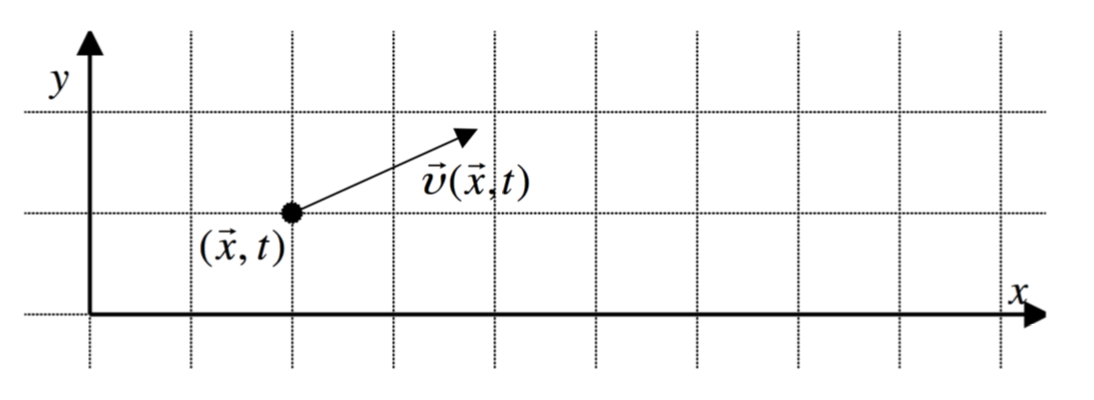
\includegraphics[scale = 0.4]{Figures/grid_method.png}
        \caption{Grid description, $retrieved from MIT(2011)$}
    \end{figure}

\section{Smoothed Particle Hydrodynamics}
    Smoothed particle hydrodynamics (SPH) was invented to simulate nonaxisymmetric phenoma in astrophysis initially. The principal idea of SPH is to treat hydrodynamics in a completely mesh-free fashion, in terms of a set of sampling particles. It turns out that the particle presentation of SPH has excellent conservation properties. Energy, linear momentum, angular momentum, mass and velocity.

    \subsection{Fundamentals}

    At the heart of SPH is a kernel interpolation method which allows any function to be expressed in terms of its values at a set of disordered points - the particles\cite{monaghan1992smoothed}. For ant field $A(\textbf{r})$, a smoothed interpolated version $A_{I}(\textbf{r})$ can be defined by a kernel $W(\textbf{r}, h)$,
    \begin{equation}
        A_{I}(\textbf{r}) = \int A({\textbf{r}}^{\prime})W(\|\textbf{r} - \textbf{r}^{\prime}\|, h)\dif\textbf{r}^{\prime}
    \end{equation}
    \begin{figure}[!ht]
        \centering
        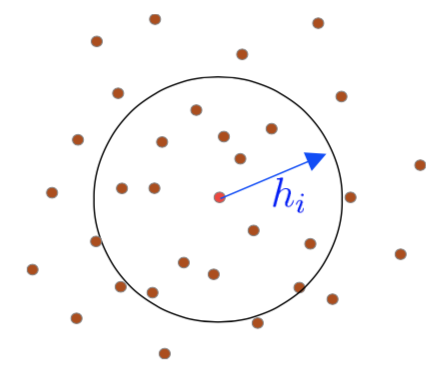
\includegraphics[scale = 0.6]{Figures/sph}
        \caption{Visilaztion of SPH}
    \end{figure}

    where the integration is over the entire space, and $W$ is an interpolating kernel with 
    \begin{equation}
        \int W(\|\textbf{r} - \textbf{r}^{\prime}\|, h)\dif \textbf{r}^{\prime} = 1
    \end{equation}
    and
    \begin{equation}
        \lim_{h\to 0} W(\|\textbf{r} - \textbf{r}^{\prime}\|, h)\dif\textbf{r}^{\prime} = \delta(\|\textbf{r} - \textbf{r}^{\prime}\|) 
    \end{equation}

    Normally, we want the kenel to be Non-negative and rotational invariant.
    \begin{equation}
        W(\|\textbf{x}_{i} - \text{x}_{j}\|, h) = W(\|\text{x}_{j} - \text{x}_{i}\|, h)
    \end{equation}

    \begin{equation}
        W(\|\textbf{r} - \textbf{r}^{\prime}\|, h) \ge 0
    \end{equation}

    For numerical work, we can use midpoint rule,
    \begin{equation}
        A_{I}(\textbf{x}) \approx A_{S}(\textbf{x}) = \sum_{i} A(\textbf{x}_{i})W(\|\textbf{x}_{i}-\textbf{x}\|, h)\Delta V_{i}
    \end{equation}
    Since $V_{i} = m_{i}/\rho _{i}$
    \begin{equation}
        A_{S}(\textbf{x}) = \sum_{i} \frac{m_{i}}{\rho_{i}} A(\textbf{x}_{i})W(\|\textbf{x}_{i}-\textbf{x}\|, h)
    \end{equation}

    The default, gradient and Laplacian of $A$ are:
    \begin{equation}
        \begin{aligned}
            \nabla A_{S}(\textbf{x}) &= \sum_{i} \frac{m_{i}}{\rho_{i}} A(\textbf{x}_{i})\nabla W(\|\textbf{x}_{i}-\textbf{x}\|, h) \\
            \nabla^{2} A_{S}(\textbf{x}) &= \sum_{i} \frac{m_{i}}{\rho_{i}} A(\textbf{x}_{i})\nabla^{2} W(\|\textbf{x}_{i}-\textbf{x}\|, h)
        \end{aligned}
        \label{eq:1}
    \end{equation}

    \subsection{Kernels}
    Smoothing kernels functions are one of the most important points in SPH. Stability, accurancy and speed of the whole method depends on these fuctions. Different kernels are being used for different purposes. One possibilyty for $W$ is a Gaussian. However, most current SPH implementations are based on kernels with finite support. We mainly introduce gaussian, poly6 and spicky kernel here. And compare the different kernels and their property.

    \subsubsection{Poly6}
    The kernel is also known as the 6th degree polynomial kernel.
    \begin{equation}
        W_{poly 6}(\textbf{r}, h) = \frac{315}{64\pi h^{9}}
            \begin{cases}
                (h^2 - \|\textbf{r}\|^2)^3 & 0 \le \|\textbf{r}\| \le h \\
                0 & \textrm{Otherwise}
            \end{cases}
    \end{equation}

    Then, the gradient of this kernel function can be
    \begin{equation}
        \nabla W_{poly 6}(\textbf{r}, h) = - \frac{945}{32\pi h^9}
            \begin{cases}
                \textbf{r}(h^2 - \|\textbf{r}\|^2)^2 & 0\le\|\textbf{r}\|\le h \\
                0 & \textrm{Otherwise}\\
            \end{cases}
    \end{equation}

    The laplacian of this kenel can be expressed by, 
    \begin{equation}
        \nabla^2 W_{poly6}(\textbf{r}, h) = - \frac{945}{16\pi h^9}
            \begin{cases}
                (h^2 - \|\textbf{r}\|^2)(3h^2-7\|\textbf{r}\|^2) & 0\le\|\textbf{r}\|\le h \\
                0 & \textrm{Otherwise}\\
            \end{cases}
    \end{equation}

    \subsubsection{Spicky}

    The kernel proposed by Desbrum\cite{desbrun1996smoothed}
    \begin{equation}
        W_{spiky}(\textbf{r}, h) = \frac{15}{\pi h^6}
            \begin{cases}
                (h - \|\textbf{r}\|)^3 & 0\le\|\textbf{r}\|\le h \\
                0 & \textrm{Otherwise}\\
            \end{cases}
    \end{equation}

    Then, the gradient of spiky kernel can be described by,
    \begin{equation}
        \nabla W_{spiky}(\textbf{r}, h) = -\frac{45 \textbf{r}}{\pi h^6 \|\textbf{r}\|}
            \begin{cases}
                (h - \|\textbf{r}\|)^2 & 0\le\|\textbf{r}\|\le h \\
                0 & \textrm{Otherwise}\\
            \end{cases}
    \end{equation}
     The laplacian of spiky can be expressed by,
     \begin{equation}
        \nabla^2 W_{spiky}(\textbf{r}, h) = \frac{90}{\pi h^6}
            \begin{cases}
                h - \| \textbf{r} \| & 0 \le \| \textbf{r} \| \le h \\
                0 & \textrm{Otherwise}\\
            \end{cases}
    \end{equation}

    \begin{figure}[!ht]
        \centering
        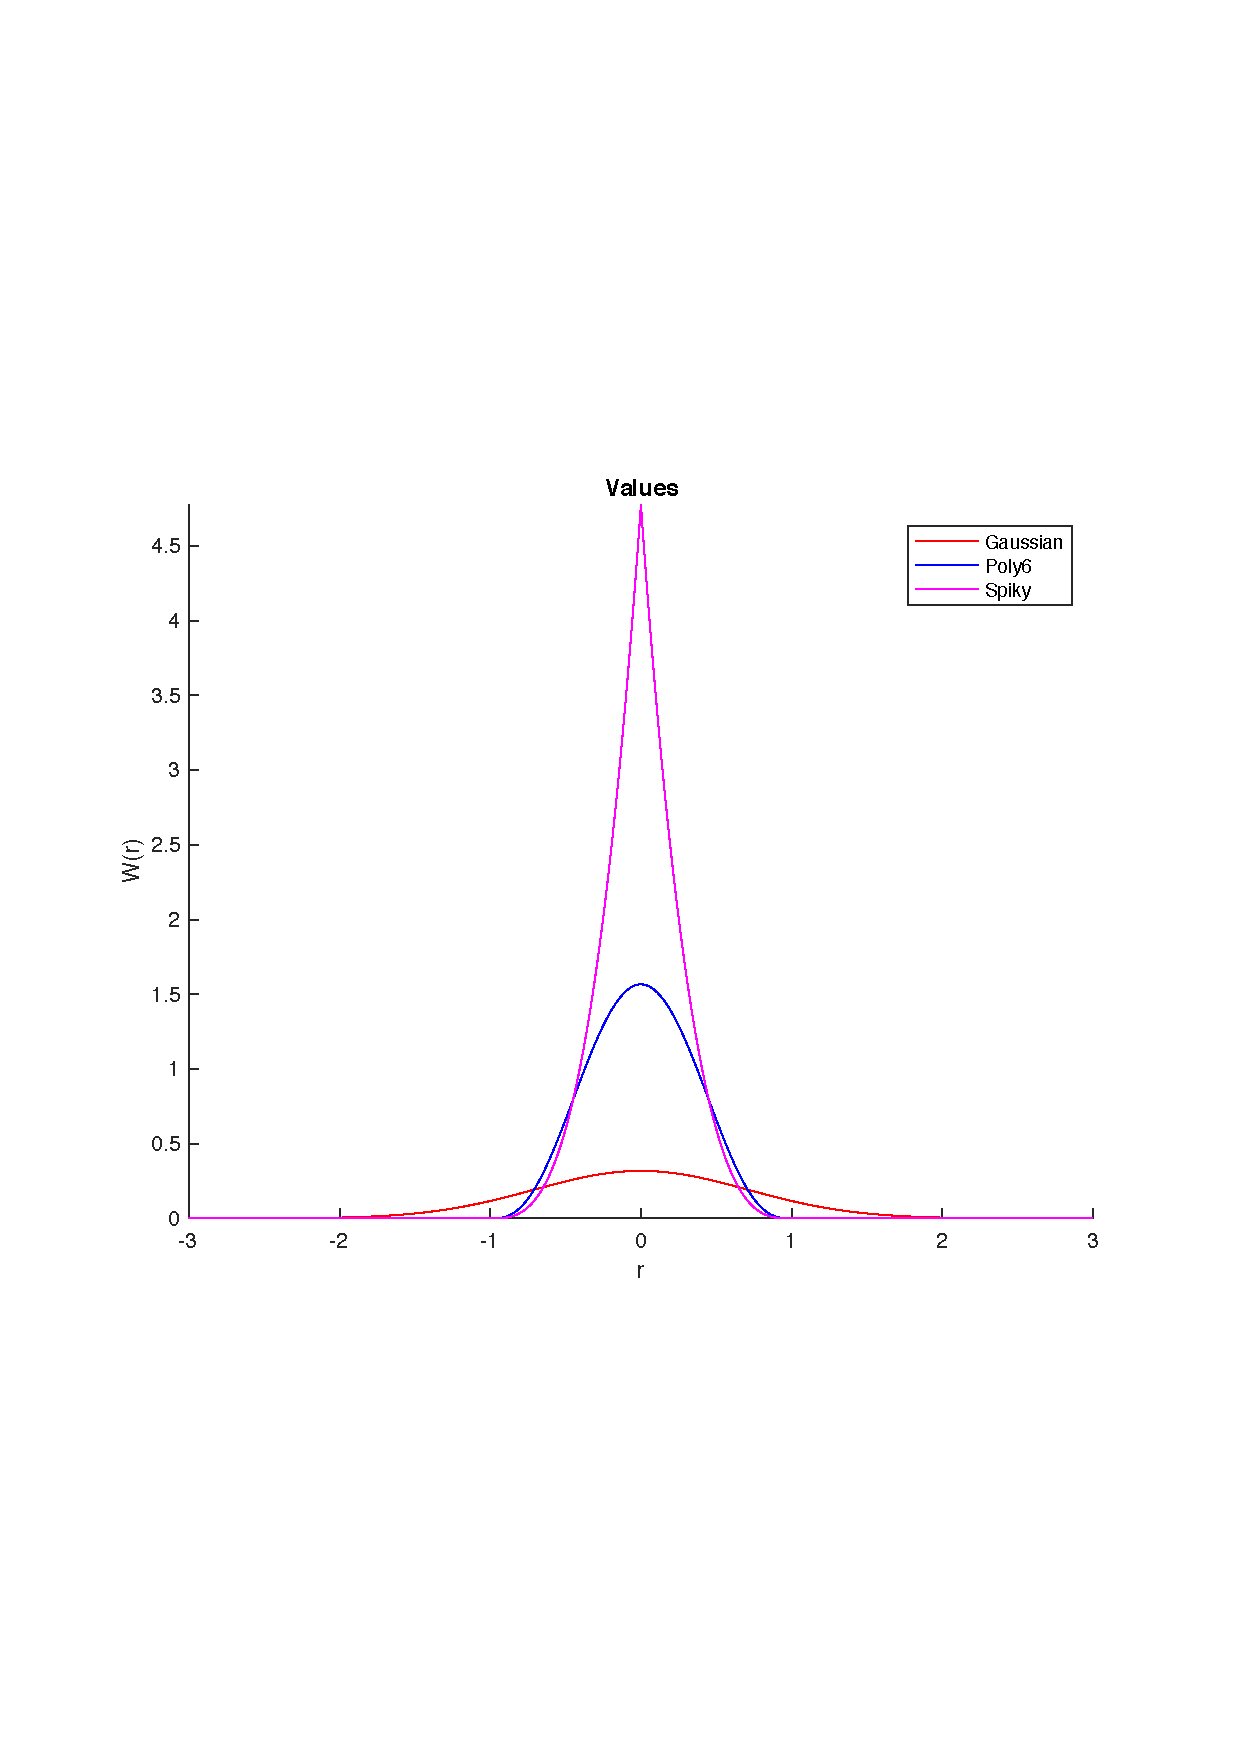
\includegraphics[scale = 0.5]{Figures/kernels}
        \caption{Comparation of different kernels, we set smoothing length $h = 1$ here.}
    \end{figure}

    \begin{figure}[!ht]
        \centering
        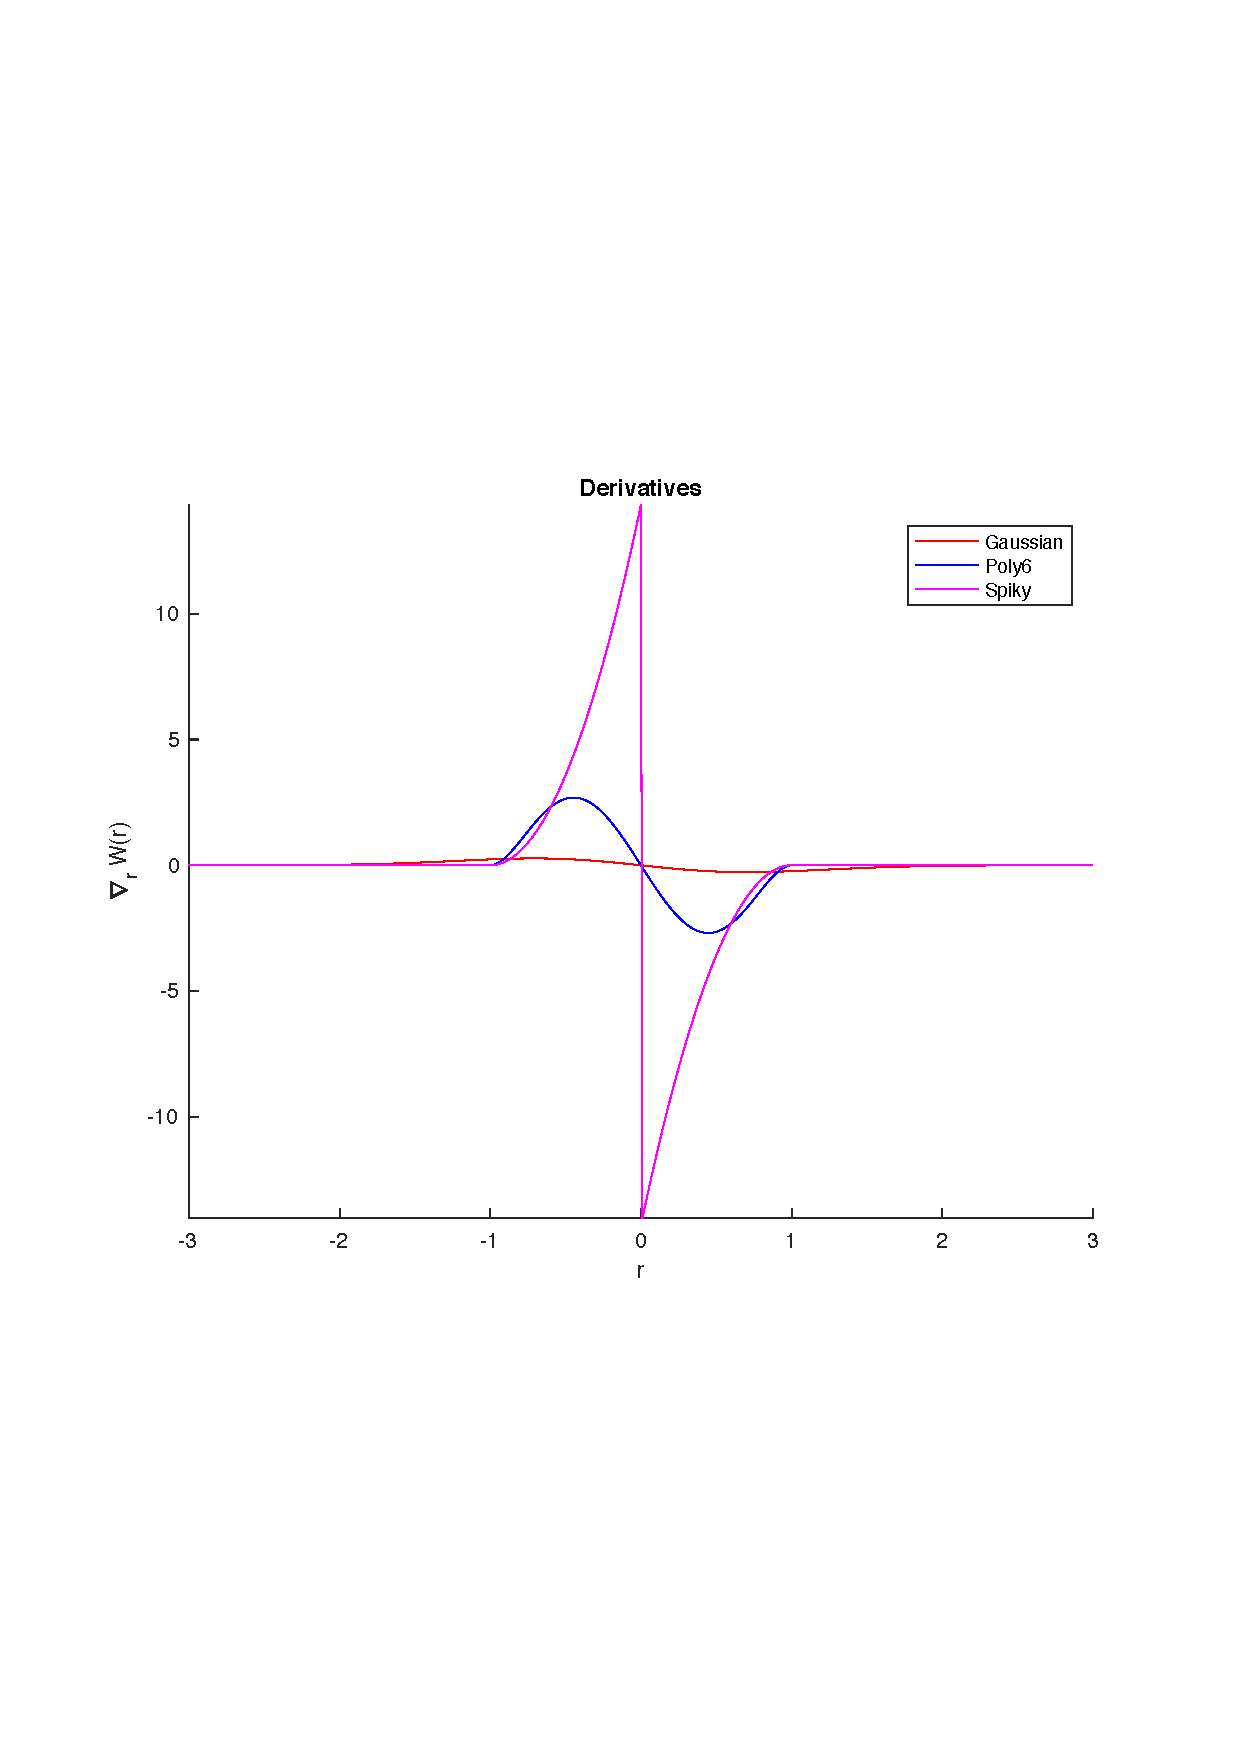
\includegraphics[scale = 0.5]{Figures/kenels_de}
        \caption{Comparation of gradient of different kernels, we set $h = 1$ here. }
    \end{figure}

    \subsection{Grid size and smoothing length}

    The grid should be also fine enough to capture the variation in our simulation. In our case, it is reasonable to have a grid fine enough such that no two contact points are mapped into the same cell. \\

    Smoothing length, $h$, is one of the most important parameters that affects the whole SPH method by changing the kernel value results abd neighbor searching results. Too small or too big values might cause lose essencail information in the simulation.

    \subsection{Neignbor Search}
    Neighbor search is one of the most crucial procedures in SPH method considersing all interpolation equations, $A(\textbf{r})$, needs the neighbor list for every particle (refer to equation \ref{eq:1}). A naive neighbor searching approach would end up with a complexity of $o(n^2)$. The complexity is not good enough since it is impossoble to reach any interactive speed when the particle count increses. With an efficient nearest neighbor searching(NNS) algorithm, it is possible to have a significant performance increase since it is the most time consuming procedure in SPH computation. In order to decrease the complexity, we choose to use $k-d$ tree data structure to store the particla spatial information and then do the nearest neighbor searching.

        \subsubsection{Hierarchical Tree}
        Using an adaptive hierarchy tree search is proposed by Paiva\cite{paiva2006particle} to find particle neighbors. Since the simulation takes place in two dimensions, $k-d$ tree data structure was used in this approach. \\

        An octree structure has been adapted from Macey (b) Octree Demo. The hierarchy tree is formed with a pre-defined height. The simulation box is divided recursively into eight pieces, nodes. The nodes at height = 1 are called leaves. Each node has a surrounding box for particle query which is used to check if the particle is inside the node. Each parent node, contains the elements that are divided through its children. The particle is being checked at each level of the tree if it’s intersecting the node. If it does, descend one level down in that node. After reaching to leaves, bottom level, particle has been checked if its within the search distance, $h$. If the particle is in the range, add it to the neighbor list. Neighbor searching is done when the whole tree has been traversed. The search distance set to be smoothing length in this implementation. \\

        The complexity of this tree search method is $O(nlog(n))$, n being the number of particles. The performance of this algorithm is worse than Spatial Hashing method. In addition, the results obtained using this NNS algorithm wasn’t accurate and stable for this implementation. Therefore as mentioned above, Spatial Hashing method was preferred.


\section{Grid to particle}
    After getting the grid image for simulation state in $t$, we will use the grid cells as input and renew the grid image based on trained model. Once the grid image in $t+\delta t$ have been renewed, the next step is to transfer the grid to particles which will instore all information including velocity,  
    \subsection{interpolation}
    \begin{figure}[!ht]
        \centering
        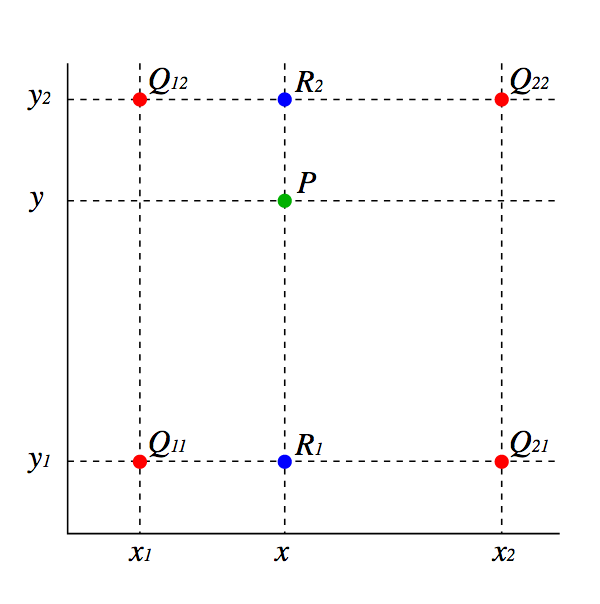
\includegraphics[scale = 0.5]{Figures/inp}
        \caption{Comparation of gradient of different kernels, we set $h = 1$ here. }
    \end{figure}
    We first do linear interpolation in the $x$-direction. This yields

    \begin{equation}
        \begin{aligned}
            (x,y_{1})&\approx {\frac {x_{2}-x}{x_{2}-x_{1}}}f(Q_{11})+{\frac {x-x_{1}}{x_{2}-x_{1}}}f(Q_{21}),\\f(x,y_{2})&\approx {\frac {x_{2}-x}{x_{2}-x_{1}}}f(Q_{12})+{\frac {x-x_{1}}{x_{2}-x_{1}}}f(Q_{22}).
        \end{aligned}
    \end{equation}

    \begin{equation}
        \begin{aligned}f(x,y)&\approx {\frac {y_{2}-y}{y_{2}-y_{1}}}f(x,y_{1})+{\frac {y-y_{1}}{y_{2}-y_{1}}}f(x,y_{2})\\&={\frac {y_{2}-y}{y_{2}-y_{1}}}\left({\frac {x_{2}-x}{x_{2}-x_{1}}}f(Q_{11})+{\frac {x-x_{1}}{x_{2}-x_{1}}}f(Q_{21})\right)\\+{\frac {y-y_{1}}{y_{2}-y_{1}}}\left({\frac {x_{2}-x}{x_{2}-x_{1}}}f(Q_{12})+{\frac {x-x_{1}}{x_{2}-x_{1}}}f(Q_{22})\right)\\&={\frac {1}{(x_{2}-x_{1})(y_{2}-y_{1})}}{\big (}f(Q_{11})(x_{2}-x)(y_{2}-y)+f(Q_{21})(x-x_{1})(y_{2}-y)+f(Q_{12})(x_{2}-x)(y-y_{1})+f(Q_{22})(x-x_{1})(y-y_{1}){\big )}\\&={\frac {1}{(x_{2}-x_{1})(y_{2}-y_{1})}}{\begin{bmatrix}x_{2}-x&x-x_{1}\end{bmatrix}}{\begin{bmatrix}f(Q_{11})&f(Q_{12})\\f(Q_{21})&f(Q_{22})\end{bmatrix}}{\begin{bmatrix}y_{2}-y\\y-y_{1}\end{bmatrix}}.\end{aligned}
    \end{equation}

\section{Conclution}